\documentclass[a4paper,12pt]{article}

\usepackage{url}
\usepackage{amsmath}
\usepackage{amssymb}
\usepackage{epsfig}
\usepackage{mathtools}
\usepackage{graphics}
\usepackage{fancyhdr}
\usepackage{cite}
\usepackage{algorithm}
\usepackage[noend]{algpseudocode}

\usepackage{color}
\usepackage{colortbl}
\definecolor{LightGray}{gray}{0.9}

\graphicspath{{pictures/}}

\title{Report for assignment 1 in the course DD2438 at KTH}
\author{\hspace*{-0.5cm}
GROUP10\\
\begin{tabular}{cccc}
Arash Safari & Ermias Gebremeskel \\
%BIRTHDATE1 & BIRTHDATE2 \\
asafari@kth.se & ermiasg@kth.se \\
%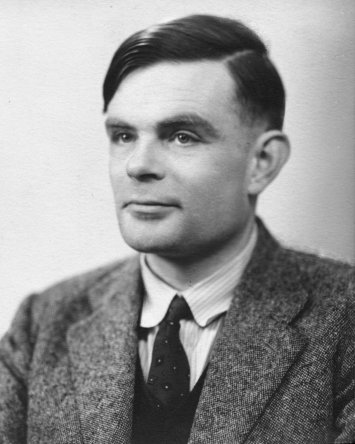
\includegraphics[width=0.13\linewidth]{Alan_Turing_photo} & 
%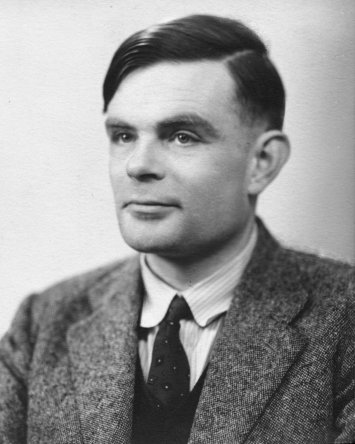
\includegraphics[width=0.13\linewidth]{Alan_Turing_photo}
\end{tabular}} 
\date{}

\pagestyle{fancy}
\setlength{\headheight}{15pt}
\fancyhf{}
\lhead{DD2438 agent16} % DO NOT REMOVE!!!!
\rhead{Arash Safari, Ermias Gebremeskel} %% UPDATE WITH YOUR NAMES
\begin{document}

\maketitle
\thispagestyle{fancy}

\begin{abstract}
This paper will discuss autonomous system motion models including path following and path planing algorithms for these models. This is done by researching and implementing four motion models to simulate the movement of objects in a frictionless two dimensional space and then find a working path following and planing algorithms for these models. The final implementation includes motion models for discrete, kinematic (point and car), dynamic (point and car), and differential drive, with a simple path finding algorithm that takes two points (start and target) and attempt to steer an object to its target. The paths for the models were manly constructed using two algorithms: visibility graphs and rapidly exploring random tree (RRT). Visibility graph was shown to perform better for the models with only two dimensions (x and y), only being outperformed by RRT when extra dimensions are involved.  
 
\end{abstract}



\clearpage

%%%%%%%%%%%%%%%%%%%%%%%%%%%%%%%%%%%%%%%%%%%%%%%%%%%%%%%%%%%%%
%%%%%%%%%%%%%%%%%%%%%%%%%%%%%%%%%%%%%%%%%%%%%%%%%%%%%%%%%%%%%
\section{Introduction}
\label{sec:intro}

One of the most fundamental cornerstones of autonomous mobile robots is navigation. It is after all perfectly reasonable to expect a 'mobile' robot to be mobile. Unfortunately, it is not always simple to guarantee this feature. Different units with different physical properties move under different constraints. And the interaction with obstacles in the environment introduces an additional level of complexity. Even though this field is rather well explored, and great advances has been made to the point where self-driving cars already is a reality, there still is room for improvement. In this report, we will describe our work done during the first assignment of the DD2438 course, which mainly focuses on navigation of units with varying properties in an obstacle filled area. The purpose of this assignment is to gain an understanding of the theory by studying and implementing existing algorithms and methods.

More specifically, the work that the report describes focuses on generating a path through the obstacle filled area that the unit could follow. This is referred to as 'Path Planning' and is achieved through various algorithms such as Visibility graphs and RRT, which we will describe and compare in detail during the report. The nature and complexity of these generated paths are dependent on the motion model of the units, which is a term for describing the limitation of which the unit was allowed manoeuvre under. The motion models that were explored in this assignment were Discrete, Kinematic and dynamic point models, differential drive model, and Kinematic and Dynamic car models. All of which will be described in more detail in the following chapters. The area that the units needed to navigate through contained non-convex polygon-shaped obstacles. 

\subsection{Contribution}
This project is done as an assignment in an introductory course in robotics and does not have any real contribution to the field of robotics. All the algorithms discussed and implemented here are solutions that can be found in many robotics and path planing books. The report will hopefully be useful to any novice in the field seeking an introduction to how different path planning algorithms can be used to navigate to a destination through obstacles. 
   

\subsection{Outline}
This report is divided in three sections. Section~\ref{sec:relwork} will cover the theoretical part of the work. Motion models and how we can model continues systems in a discrete manner is discussed in Section~\ref{sec:mm}. Section~\ref{sec:pp} will then discuss path planning algorithms. In Section~\ref{sec:method} the implementation details and how the theory discussed in Section~\ref{sec:relwork} is put to practice is described in some detail. Finally the results of some experiments will be presented before concluding the report with our conclusions in Section~\ref{sec:exps}.
 

%%%%%%%%%%%%%%%%%%%%%%%%%%%%%%%%%%%%%%%%%%%%%%%%%%%%%%%%%%%%%
%%%%%%%%%%%%%%%%%%%%%%%%%%%%%%%%%%%%%%%%%%%%%%%%%%%%%%%%%%%%%

\section{Related work}
\label{sec:relwork}
In this Section, the theoretical back ground needed to understand this paper and a short description of few related works that we found useful before and during the implementation of our solutions are discussed.
\subsection{Motion models}
\label{sec:mm}
In path following and planing the form of the robot performing the task and the environment determine the number of degrees of freedom of the system. If the robot can move instantaneously in any direction we call the robot omnidirectional(holonomic constrained) on the other hand if the robot have velocity constraints that prevent it from instantaneously changing direction the robot is called nonholonomic. Besides the degree of freedom a robot can also be modelled by kinematic equations, using velocities as controls or by dynamic equations, using forces as controls. \cite{lynch_principles_2005}    
 
 In this project we are simulating six motion models, three of which are holonomic and three nonholonomic. We start by analysing the simpler holonomic models: discrete, kinematic point, and dynamic point models. Then we will try to build up to the nonholonomic ones: differential drive, kinematic car, and dynamic car models. 
 
 \begin{itemize}
\item \textbf{Discrete point}. In this model all the control does is take the position of the robot and move it's $x$ and $y$ coordinates with a predefined minimum step in order for the robot to end-up at it's desired position.  
\begin{align*}
x_{k+1} &= x_{k} + a\\
y_{k+1} &= y_{k} + b
\end{align*}

Where $(x,y)$ represent a point in the coordinate system and $a$ and $b$ represent the number of steps the robot takes in $x$ and $y$ direction respectively. 

\item \textbf{Kinematic point model}. Here velocities are used as controls. The position of the robot is not set directly like in the discrete point model but rather as a velocity vector. This will give us a smother model that does not jump from point to point.   
\begin{align*}
\dot{x} &= v_x\\
\dot{y} &= v_y
\end{align*} 
Where $\dot{x}$ and $\dot{y}$ are the velocities in the respective directions, and $v_x$ can be calculated using numerical integration of ordinary differential equations $(x_{k+1} - x_{k}) / dt$.
\item \textbf{Dynamic point model}. Even though kinematic models can give us a smother movement it is still physically impossible to change velocity instantaneously. In reality movement is controlled by forces and dynamic models simulate this by controlling robots via forces instead of velocity.  
\begin{align*}
\ddot{x} &= F_x/m \\
\ddot{y} &= F_y/m
\end{align*}
Where $\ddot{x}$ and $\ddot{y}$ are the accelerations acting on the $x$ and $y$ directions, and $F/m$ can be calculated using numerical integration by setting initial $V_0 = 0$.
  
\item \textbf{Differential drive}. Is a nonholonomic robot with three degrees of freedom $(x,y)$ position and $\theta$ orientation. As in kinematic model velocity is used as a control for differential drive model. 
\begin{align*}
\dot{x} &= v\cos\theta\\
\dot{y} &= v\sin\theta\\
\dot{\theta} &= \omega
\end{align*}  

\item \textbf{Kinematic car}. As in kinematic point model the car model is controlled by velocity but with orientation $\theta$ and a length $L$ that represent the length of the car. Unlike the differential drive model a car model can not turn on the spot thus the rotational velocity($\dot{\theta}$) is constrained both by the velocity and length of the car.    
\begin{align*}
\dot{x} &= v\cos\theta\\
\dot{y} &= v\sin\theta\\
\dot{\theta}& = \frac{v}{L}\tan\phi
\end{align*}  

\item \textbf{Dynamic car}. The only difference between kinematic car and dynamic car is that the dynamic car is controlled by force as mentioned previously. Thus the equation for the dynamic car motion model is given by: 
\begin{align*}
\dot{x} &= v\cos\phi\\
\dot{y} &= v\sin\phi\\
\dot{\theta}& = \frac{v}{L}\tan\phi\\
\dot{v} &= F/m
\end{align*}  

\end{itemize} 

\subsection{Visibility Graphs} 
\label{sec:vg}
The visibility graph\cite{berg_visibility_2000} in the Euclidean plane with polygon obstacle is a graph whose nodes corresponds to the corners of the polygon, and whose edges connect the nodes that can be reached with out crossing a polygon. The visibility graph can then be used to find an optimal path with a graph search algorithm. Visibility graphs are efficient for point models, but for models with higher degree of freedom they do not scale. 

 
\subsection{Rapidly-exploring Random Trees} 
\label{sec:rrt}
Rapidly-exploring Random Trees \cite{lavalle1998rapidly} is an incremental method to quickly explore an entire system of configuration of a model. RRT do not produce an optimal solution but because they can find random path very quickly we can run them multiple times to fine a better path.  

\subsection{“Overview of motion planning”  by Matt Klingensmith}
\label{sec:pp}
Although this is not an academic work, it could be described as a compilation of such works, described and explained extremely pedagogically. The Article is written by Matt Klingensmith, a robotic researcher and covers everything from the basics of motion planning such as the 'Bug algorithm' all the way down to the more recent discoveries such as RRT* and everything in-between. 
The relevant parts of this article that was of most use to us were the sections about Visibility graphs and RRT. In these sections, the advantages, disadvantages, strengths and weaknesses of these algorithms were covered.
%%%%%%%%%%%%%%%%%%%%%%%%%%%%%%%%%%%%%%%%%%%%%%%%%%%%%%%%%%%%%
%%%%%%%%%%%%%%%%%%%%%%%%%%%%%%%%%%%%%%%%%%%%%%%%%%%%%%%%%%%%%
\section{Implementation}
\label{sec:method}
This project was implemented in Java using v-rep as a simulation tool. In this section we will discuss how the different components of the project discussed in the previous section are implemented in algorithmic therms and how they were simulated.  
\subsection{Motion model implementation}
\label{sec:mmImpl}
The motion models were implemented in code exactly as the equations shown in Section~\ref{sec:mm}. By defining a frame rate $dt$ the new positions for $(x,y)$ were calculated as $x = \dot{x} * dt$ and $y = \dot{y} * dt$ respectively. 

\subsection{Path following}
\label{sec:pf}

Path following is an important part of an autonomous robot. Given a start and target points an autonomous robot needs to be capable of following the shortest path to the target. The algorithm used for path following in this project is a form of Craig Reynolds (http://www.red3d.com/cwr/) algorithmic steering behaviours for animated characters. In Craig Reynolds path-following algorithm the steering force is calculated by\\ $steering\ force = desired\ velocity - current\ velocity$ \\ and steering force is only applied if the robot stray more than a given radius from the path. The target in this algorithm is not the end of the path but any point on the path that lies on a straight line between two points on the path. In the version implemented in this project the path contains points that are relatively close and so the steering force is applied for every path point. 


		\begin{algorithm}
			\caption{Path following}
			\label{PathFollowing}
			\begin{algorithmic}[1]
				\Procedure{Path\textendash Following}{}
				\For{each point $p$ : $Path$ }
				\State $\theta = angle(position, p)$
				\State $move(p, \theta)$
				\While {$checkPoint(position, p)$}//check if check point reached
				\State $move(p, \theta)$
				\EndWhile
				\EndFor
				\EndProcedure
			\end{algorithmic}
		\end{algorithm}
		
The method $checkPoint(a,b)$ checks if the robot is with in a given radius of the check point and move tries to apply the necessary force depending on the model to steer the robot to the target. The problem with this algorithm is it does not take in to consideration the velocity of the robot, and if it can not get to the target with it's current velocity it will go in circles until it gets close enough to the check point.

\subsection{Path Finding}
\label{sec:pfinding}

As mentioned earlier, the properties of the motion model is a big factor when finding a path. As the complexity of the motion models increases, so does the nature of the path finding algorithm.
While there are universal algorithms that can be adapted to operate with any given motion model, such as RRT*, the implementation and execution costs can not easily be justified for simpler motion models.

In our project, we implemented different path finding algorithms for different types of motion models. We will now go through these different algorithms.

\subsection{Discrete Map}
\label{sec:dm}
The simplest type of motion model is the discrete motion model, where the unit can simply change its position from the current one to any one of the valid neighbours.
This motion model had to navigate through a grid like map where certain cells were marked as occupied.
In order to find a path through this map, the map was represented through a adjacency graph. An optimal path could then be calculated through the usage of the A* algorithm.
\subsection{Polygon Map}
\label{sec:pm}
The polygon map is not as straight forward as the simple discrete map. This map can not as easily be represented through a simple grid system without complications. Instead, we chose to represent the polygonal obstacles through Line2D objects in  Java. We could thereby calculate collisions between the trajectory of the unit and the obstacles through the usage of the 'Intersects()' method of that class.
\subsection{Kinematic point model}
\label{sec:kpm}
Besides the discrete point model, the kinematic point model is the simplest model to find a path for. Since the Kinematic point model can instantly switch speed and direction at will with no constraints, it can follow a path consisting of straight lines and sharp turns.
With this in mind, we chose to use a combination of Visibility graph and A* in order to find an optimal path for this model.

\subsection{Dynamic point and Car models}
\label{sec:dpm}
When it came to the dynamic point and car models, things got more complicated. The dimensionality of the problem at hand increased with each addition feature, such as the acceleration, length, the angle of the vehicle and so on. 
There are tricks and gimmicks available to make visiblity graphs viable for these kind of models, such as virtually increasing the size of the obstacles to account for the size and turning of the car models. However, it did not feel like forcing the algorithm out of its comfort zone by overcomplicating things was a good approach. Especially when there were other algorithms such as RRT that could naturally handle the types of models we were working with without the need for additional changes to the algorithm. We therefore decided to implement RRT for the Dynamic point and Car models.
While the RRT algorithm manages to find paths at a relatively rapid pace, the paths tend to be suboptimal. There are ways to counteract this by for example implementing the RRT* version of the algorithm, which guarantees optimality at the cost of computation time and implementation complexity. However, we decided to instead take advantage of the features of the plain RRT algorithm, namely its speed and randomness, in order to produce close to optimal paths,
The idea was to further optimize the running time of our RRT algorithm with the help of heuristics. By doing so, we would be able to generate a high number of possible paths quickly, and pick the best one. If the number of generated paths were to be high enough, we figured that the best ones should be comparable to an optimal path.
In order to speed up the running time, or in other words, find a valid path quickly, several different strategies and heuristics were tested.  
The first one we tried was to instead of sampling a completely random point in the map, to instead sample the goal at a certain frequency. While this heuristic was important in order for the algorithm to find a path, it usually led to a large number of branches crashing right into an obstacle in search for the goal. The generation of all these branches not only redundant, but also over crowded the tree, causing searching through the tree to take longer as time passed.
From this, we concluded that sampling the goal node while not having clear sight of it does little else than directing the flow of the graph towards the goal node, which it also does inefficiently. 
An alternative that we decided to try out instead was to make the tree spread broadly and rapidly, until it has a clear view of the goal node. At that point, we can start sampling the goal point.
In order to make the tree spread widely and rapidly, we had to experiment with a set of variables such as speed range, turn range and sample range. 
The combination of methods  that turned out to be most successful in our case was:
 \begin{itemize}
\item Maximum speed at all times
\item Reducing the Maximum allowed turning angle to 30\%
\item Do not turn at all 60\% of the time
\item Sample the same point 5 times in a row before randomly choosing a new sample
\item With these conditions, the tree usually spreads rapidly in all directions before finding and focusing 
\item its attention towards the goal.
 \end{itemize}


%%%%%%%%%%%%%%%%%%%%%%%%%%%%%%%%%%%%%%%%%%%%%%%%%%%%%%%%%%%%%
%%%%%%%%%%%%%%%%%%%%%%%%%%%%%%%%%%%%%%%%%%%%%%%%%%%%%%%%%%%%%
\section{Experimental results}
\label{sec:exps}


\subsection{Experiemntal setup}
The experiments began with reading the specifications of the map from a file. This included the position of the obstacles, their shapes and the poistion of the start/finish points.
The polygonial obstacles were then represented through a collection of Line2D objects and stored.
At this point, the RRT algorithm sets in. It starts by adding the starting point to the tree as the root node. A random point in the map is then randomly sampled, and the closest point in the tree to the sampled point is selected. A check is made here in order to see wheter an obstacle blocks the path between the sampled points and the node from the tree. if that is the case, a new point is sampled.
The unit is then moved from the point in the tree towards the sampled point according to the specifications of the motion model and other general hueristics.
Once any node in the tree has a clear sight of the goal node, the goal node will start being sampled with a 40\% likelihood.


\subsection{Experiment}

The experminets were run by simply setting variables to the appropriate values to the ones of the motion model. The algorithm would then run repeatedly, remembering its best result. Once a long period of time, usually 20 minutes, passed without a better path being found, the algorithm would stop.
The specifications of the different models were:
\begin{itemize}
\item Problem 11: Kinematic point model with Vmax=10
\item Problem 12: Dynamic point model with 
	\begin{itemize}
	\item 12a: Vmax=20, Amax=40
	\item 12b: Vmax=20, Amax=13
	\item 12c: Vmax=20, Amax=8
	\item 12d: Vmax=100, Amax=20
	\end{itemize}
\item Problem 13: Differential drive model with Vmax=10, Wmax=0.3
\item Problem 14: Kinematic car, Vmax=10, PhiMax=pi/4
	\begin{itemize}
	\item 14a: L=10
	\item 14b: L=30
	\item 14c: L=50
	\end{itemize}
\item Problem 15: Dynamic car, PhiMax=pi/4, Vmax=100, Amax=20
	\begin{itemize}
	\item 15a: L=10
	\item 15b: L=50
	\end{itemize}
\end{itemize}
\begin{figure}
\centering
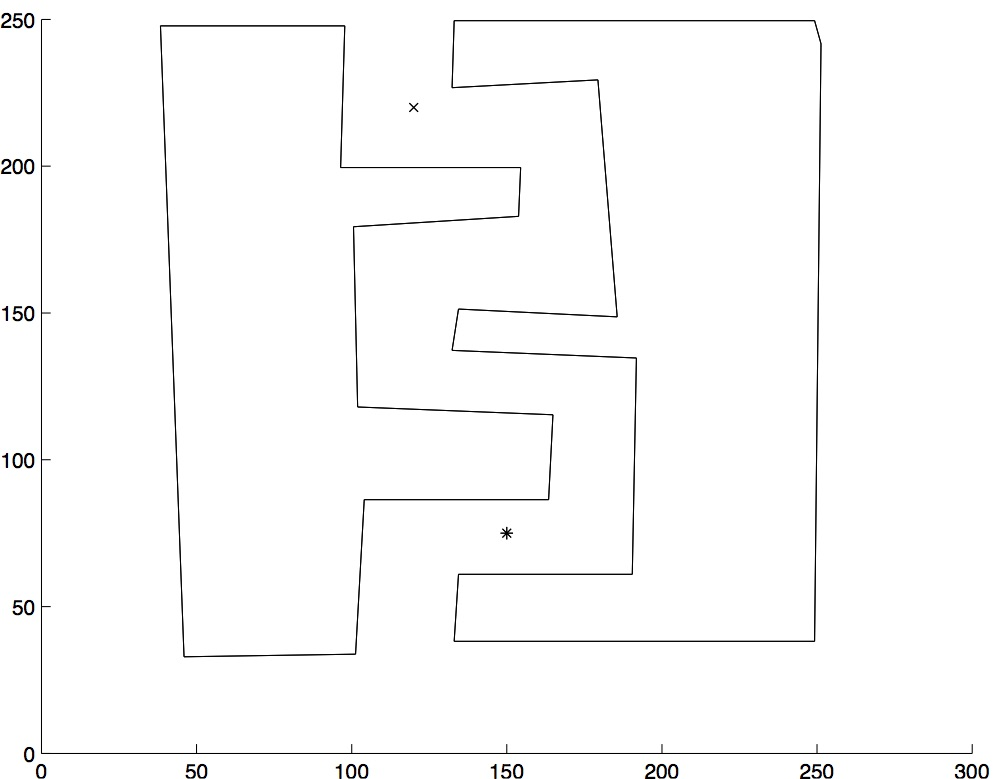
\includegraphics[width=0.8\linewidth]{polygonalMap}
\caption{The map that the units had to navigate through}
\label{fig:histogram}
\end{figure}

\subsection{Results}
The strategy described in the previous chapters worked perfectly fine for the simpler models such as the point models, and even the shorter car models.
Thousands of possible paths could be generated within a short period of time.
The best ones of these randomly generated paths were very close to the results of the other groups that did well.
However, when it came to the car models with lenghts of $ >30$, the algorithm could not find any paths at all, even when it was allowed to run for hours.

\begin{table}
    \begin{tabular}{llllllllllll}
    ~   & P11     & P12a     & P12b     & P12c     & P12d    & P13   & P14a          & P14b  & P14c  & P15a  & P15b  \\
    G1  & 19.438  & 13.3     & 15.45    & 18.97    & 12.42   & 35.66 & 28.16         & 42.48 & 62.88 & 24.14 & -     \\
    G2  & 19.63   & 17.74    & 21.77    & 26.75    & 18.49   & 37.25 & 28.16         & -     & -     & 6.00  & -     \\
    G3  & 19.93   & 13.91    & 24.28    & 27.64    & 17.74   & 37.70 & 21.14         & TBD   & TBD   & 6.80  & TBD   \\
    G4  & 19.65   & -        & 15.11    & 24.36    & -       & 30.36 & 34    & -     & -     & -     & -     \\
    G5  & 19.6    & 21.27    & ~        & ~        & ~       & 38.07 & 20.31         & ~     & ~     & 5.16  & ~     \\
    G6  & 25.17   & 19.86    & -        & -        & -       & 112.9 & 61.88         & -     & -     & -     & -     \\
    G7  & 248     & 198      & 193      & 184      & 100     & 199.5 & 191           & ~     & ~     & ~     & ~     \\
    G8  & 22      & 29       & 19       & 25       & 25      & 41.6  & 195.63        & ~     & ~     & ~     & ~     \\
    G9  & 19.69   & 13.23    & 19.69    & 24.83    & 15.44   & 46.00 & 30.75         & -     & -     & -     & -     \\ \rowcolor{LightGray}
    G10 & 19.4    & 14       & 19       & 26       & 19      & 96    & 32            & ~     & ~     & 30    & ~     \\ 
    G11 & 19.20   & 13.37    & 17.58    & 20.07    & 13.72   & 30.02 & 19.96         & 57.30 & 70.59 & 6.20  & 11.21 \\
    G12 & 20.10   & 32.58    & 35.86    & 33.82    & 30.26   & 34.52 & 23.74         & 210.3 & 220.6 & 7.97  & -     \\
    G13 & 38.19 & 33.24 & 38.74 & 38.424 & 38.96 & 36.8  & -             & -     & -     & -     & ~     \\
    \end{tabular}
\end{table}
\pagebreak
%%%%%%%%%%%%%%%%%%%%%%%%%%%%%%%%%%%%%%%%%%%%%%%%%%%%%%%%%%%%%
%%%%%%%%%%%%%%%%%%%%%%%%%%%%%%%%%%%%%%%%%%%%%%%%%%%%%%%%%%%%%
\section{Summary and Conclusions}
\label{sec:summary}
\subsection{Summary}
In summary, we tried to navigate units with different motion models, including dynamic point, dynamic car and kinematic car with the help of RRT. The paths that RRT generated, were random and therefore likely to be sub-optimal. However, due to the speed of which they were generated, we were allowed to create a great number of possible paths and pick the best one.
In most cases, this proved to be a sufficient strategy. However, when it came to cases where extreme precission was required, such as in cases where large vehicles need to navigate through small spaces, the model did not perform well.
\subsection{Conclusions}
The strategy that we adopted in our implementation proved to be successful for the test cases where precision was not vital in order to reach a goal.
In these cases, the probability of randomly arriving to the circumstances that was required for the unit to be able to traverse a choke point proved to be too small with our heuristics.
This is almost to be expected, since the main purpose of our heuristics were to spread the tree rapidly in all directions without showing too much concern for the final goal destination.
The algorithm finally turns its attention towards a goal when the goal node has been spotted. But by then, the circumstances of the node that spotted the goal, such as its position, speed and angle would usually prevent it from being able to reach the goal node. 

Group 11, which also used a plain RRT algorithm were more successful with their implementation. Their strategy was the same as our initial strategy of sampling the goal node with a certain frequency. However, they resolved the issue of the tree getting convoluted by branches that “crashed” into the obstacles by performing moves in chains of 10, and then discarding the entire chain if it crashed into an obstacle.
This was a better strategy than ours since this solved the issue of convoluted trees with redundant and unusable branches, while still retaining the advantage of focusing towards the goal during the entire running time of the algorithm.

%%%%%%%%%%%%%%%%%%%%%%%%%%%%%%%%%%%%%%%%%%%%%%%%%%%%%%%%%%%%%
%%%%%%%%%%%%%%%%%%%%%%%%%%%%%%%%%%%%%%%%%%%%%%%%%%%%%%%%%%%%%
\pagebreak
\bibliography{reflist}{}
\bibliographystyle{plain}


\end{document}